\section{Housing Assessment}

\noindent In this chapter, we document the condition, status, and needs for housing in Bloomfield. Drawing on a variety of data from the Knox County Property Assessor, various government agencies, and an original survey of Bloomfield residents, we show that Bloomfield has a long-term trend of population decline and housing structures in need of improvement. Amidst this, Bloomfield has the challenge of supporting affordable housing development while supplying amenities -- particularly childcare -- to encourage existing young families to stay in Bloomfield and new ones to move there.

\subsection{Condition of Housing Structures}

\noindent The status and condition of structures are categorized by the Knox County property assessor. \textbf{Table~\ref{table:landConditionRes}} shows how the assessor has rated these parcels in Bloomfield:

\begin{table}[H] 
\begin{framed}
\centering \doublespacing
  \caption{Bloomfield Residential Land Use Conditions}
  \label{table:landConditionRes}
 \scalebox{0.95}{
\begin{tabular}{l D{.}{.}{8.5} D{.}{.}{8.5} D{.}{.}{8.5}}
\hline \hline
& \multicolumn{1}{c}{Parcels} & \multicolumn{1}{c}{Percent of Total Parcels}  & \multicolumn{1}{c}{Perecnt of Total Area}  \\ \hline
Worn-Out                & 2     & 0.46\%    & 0.27\%    \\
Worn-Out - Badly Worn   & 2     & 0.46\%    & 0.19\%    \\
Badly Worn              & 23    & 5.29\%    & 3.58\%    \\
Badly Worn - Average    & 32    & 7.36\%    & 6.47\%    \\
Average                 & 315   & 72.41\%   & 74.99\%   \\
Average - Good          & 42    & 9.66\%    & 9.94\%    \\
Good                    & 18    & 4.14\%    & 4.00\%    \\
Good - Very Good        & 1     & 0.23\%    & 0.57\%    \\
Very Good               & 0     & 0.00\%    & 0.00\%    \\
\hline
\end{tabular}
}
\floatnote{Area units are in square miles. Data come from the Knox County Property Assessor.}
\end{framed}
\end{table}

\pagebreak
\subsubsection*{Remarks on Housing Conditions}
\begin{itemize}
    \item [(1)] \textbf{\textcolor{coBalt}{Majority of Housing is in Average Condition}}
    \begin{itemize}
        \item The most common rating for residential structures in Bloomfield is "average," indicating that:
        \begin{itemize}
            \item The majority of homes are habitable and maintain a standard level of functionality.
            \item However, they may lack modern updates or show signs of aging and general wear.
        \end{itemize}
        \item This suggests stable but aging housing stock, which may require investment in maintenance or modernization over the next decade.
    \end{itemize}
    \item [(2)] \textbf{\textcolor{coBalt}{Minimal "Worn-Out" Properties}}
    \begin{itemize}
        \item Less than one percent of homes are considered "Worn-Out," meaning:
        \begin{itemize}
            \item Very few homes are in a state of severe disrepair or uninhabitable condition.
            \item This reflects basic housing adequacy across the city, with little evidence of total structural abandonment.
            \item It also suggests that code enforcement or demolition efforts may be effective in preventing blight at the extreme end.
        \end{itemize}
    \end{itemize}
    \item [(3)] \textbf{\textcolor{coBalt}{Significant Proportion of "Badly Worn" Housing}}
    \begin{itemize}
        \item About 13\% of the housing stock is "Badly Worn, "which is a red flag:
        \begin{itemize}
            \item These homes may have serious deficiencies in systems (roofing, plumbing, electrical, foundation) or visible deterioration.
            \item This group likely represents homes that are still occupied but nearing the point where repairs or renovations are critical.
            \item This condition group is the most at-risk of becoming "Worn-Out" without intervention.
        \end{itemize}
    \end{itemize}
    \item [(4)] \textbf{\textcolor{coBalt}{Limited "Good" Condition Properties}}
    \begin{itemize}
        \item Only four percent of houses are rated as "Good" or better
        \begin{itemize}
            \item There is a small segment of housing stock that is newer, well-maintained, or recently renovated
            \item This could indicate limited recent investment in high-quality residential development or upgrades
            \item It may also highlight the need for incentives to support home improvement or new builds.
        \end{itemize}
    \end{itemize}
    \pagebreak
    \item [(5)] \textbf{\textcolor{coBalt}{Overall Implications for Housing Policy}}
    \begin{itemize}
        \item The data paint a picture of a largely functional housing stock, but one that is aging and moderately deteriorated.
        \item The low percentage of "Good" homes and the notable share of "Badly Worn" ones suggest thatBloomfield may benefit from target housing rehabilitation programs, especially for owner-occupied homes in poor condition.
        \item Grant funding and development efforts could be focused on preventing the decline of average-rated homes while prioritizing repairs for the 13\% Badly Worn stock.
    \end{itemize}
\end{itemize}

\newpage
\thispagestyle{empty}
\begin{landscape}
    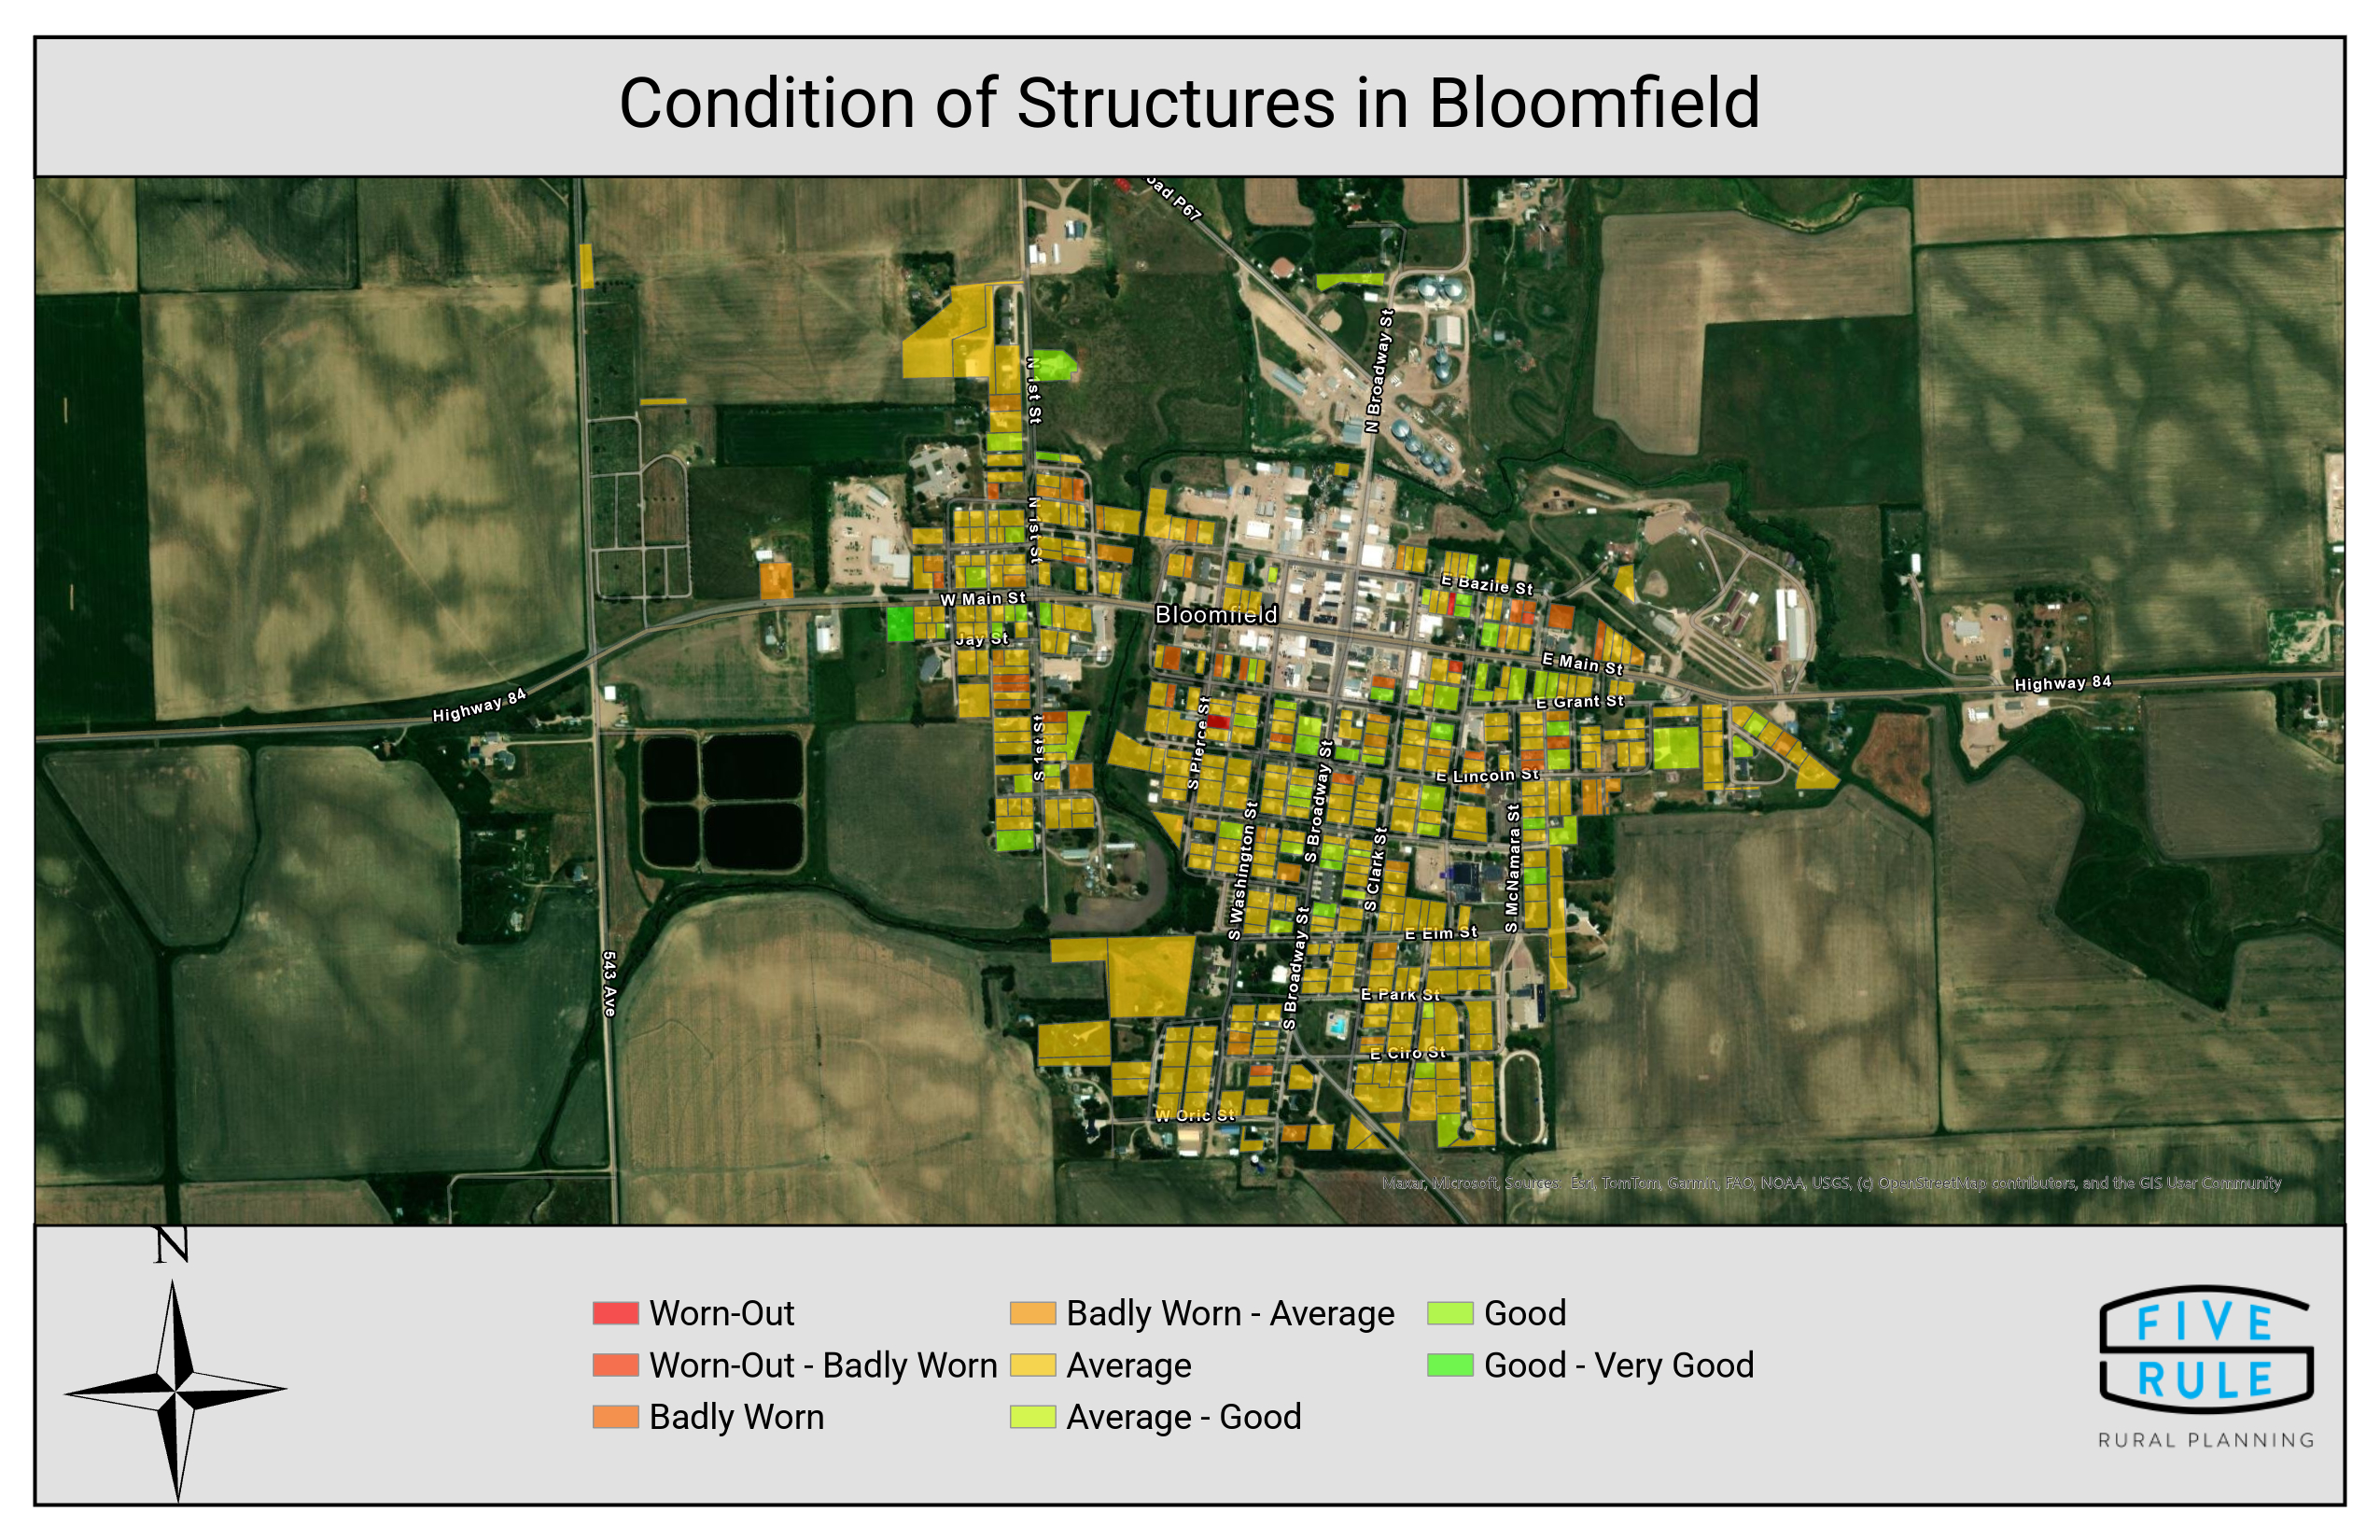
\includepdf[angle = 90]{maps/structure_conditions.pdf}
\end{landscape}
\newpage

\noindent The ages of structures are categorized by the Knox County property assessor. \textbf{Table} \hl{[]} shows the age distribution of structures in Bloomfield.\\

\noindent \hl{[need to regenerate this map]}

\pagebreak
\subsection{Vacant and Underutilized Properties}
\noindent \hl{[waiting on Scot and Brad to get back to us]}

\pagebreak
\subsection{Community Housing Needs}

% \subsubsection{Historic Population Growth and Decline}

\noindent \textbf{Figure~\ref{fig:historicPop}} shows how Bloomfield's population has changed over the last century. The city population peaked in the 1940s and experienced a smaller bump in the 1970s before beginning to steadily decline to just under 1,000 residents today. The decline was most pronounced in the 1990s.

\begin{figure}[H]
\centering
\begin{framed}
    \caption{Historic Population Growth and Decline}
    \label{fig:historicPop}
    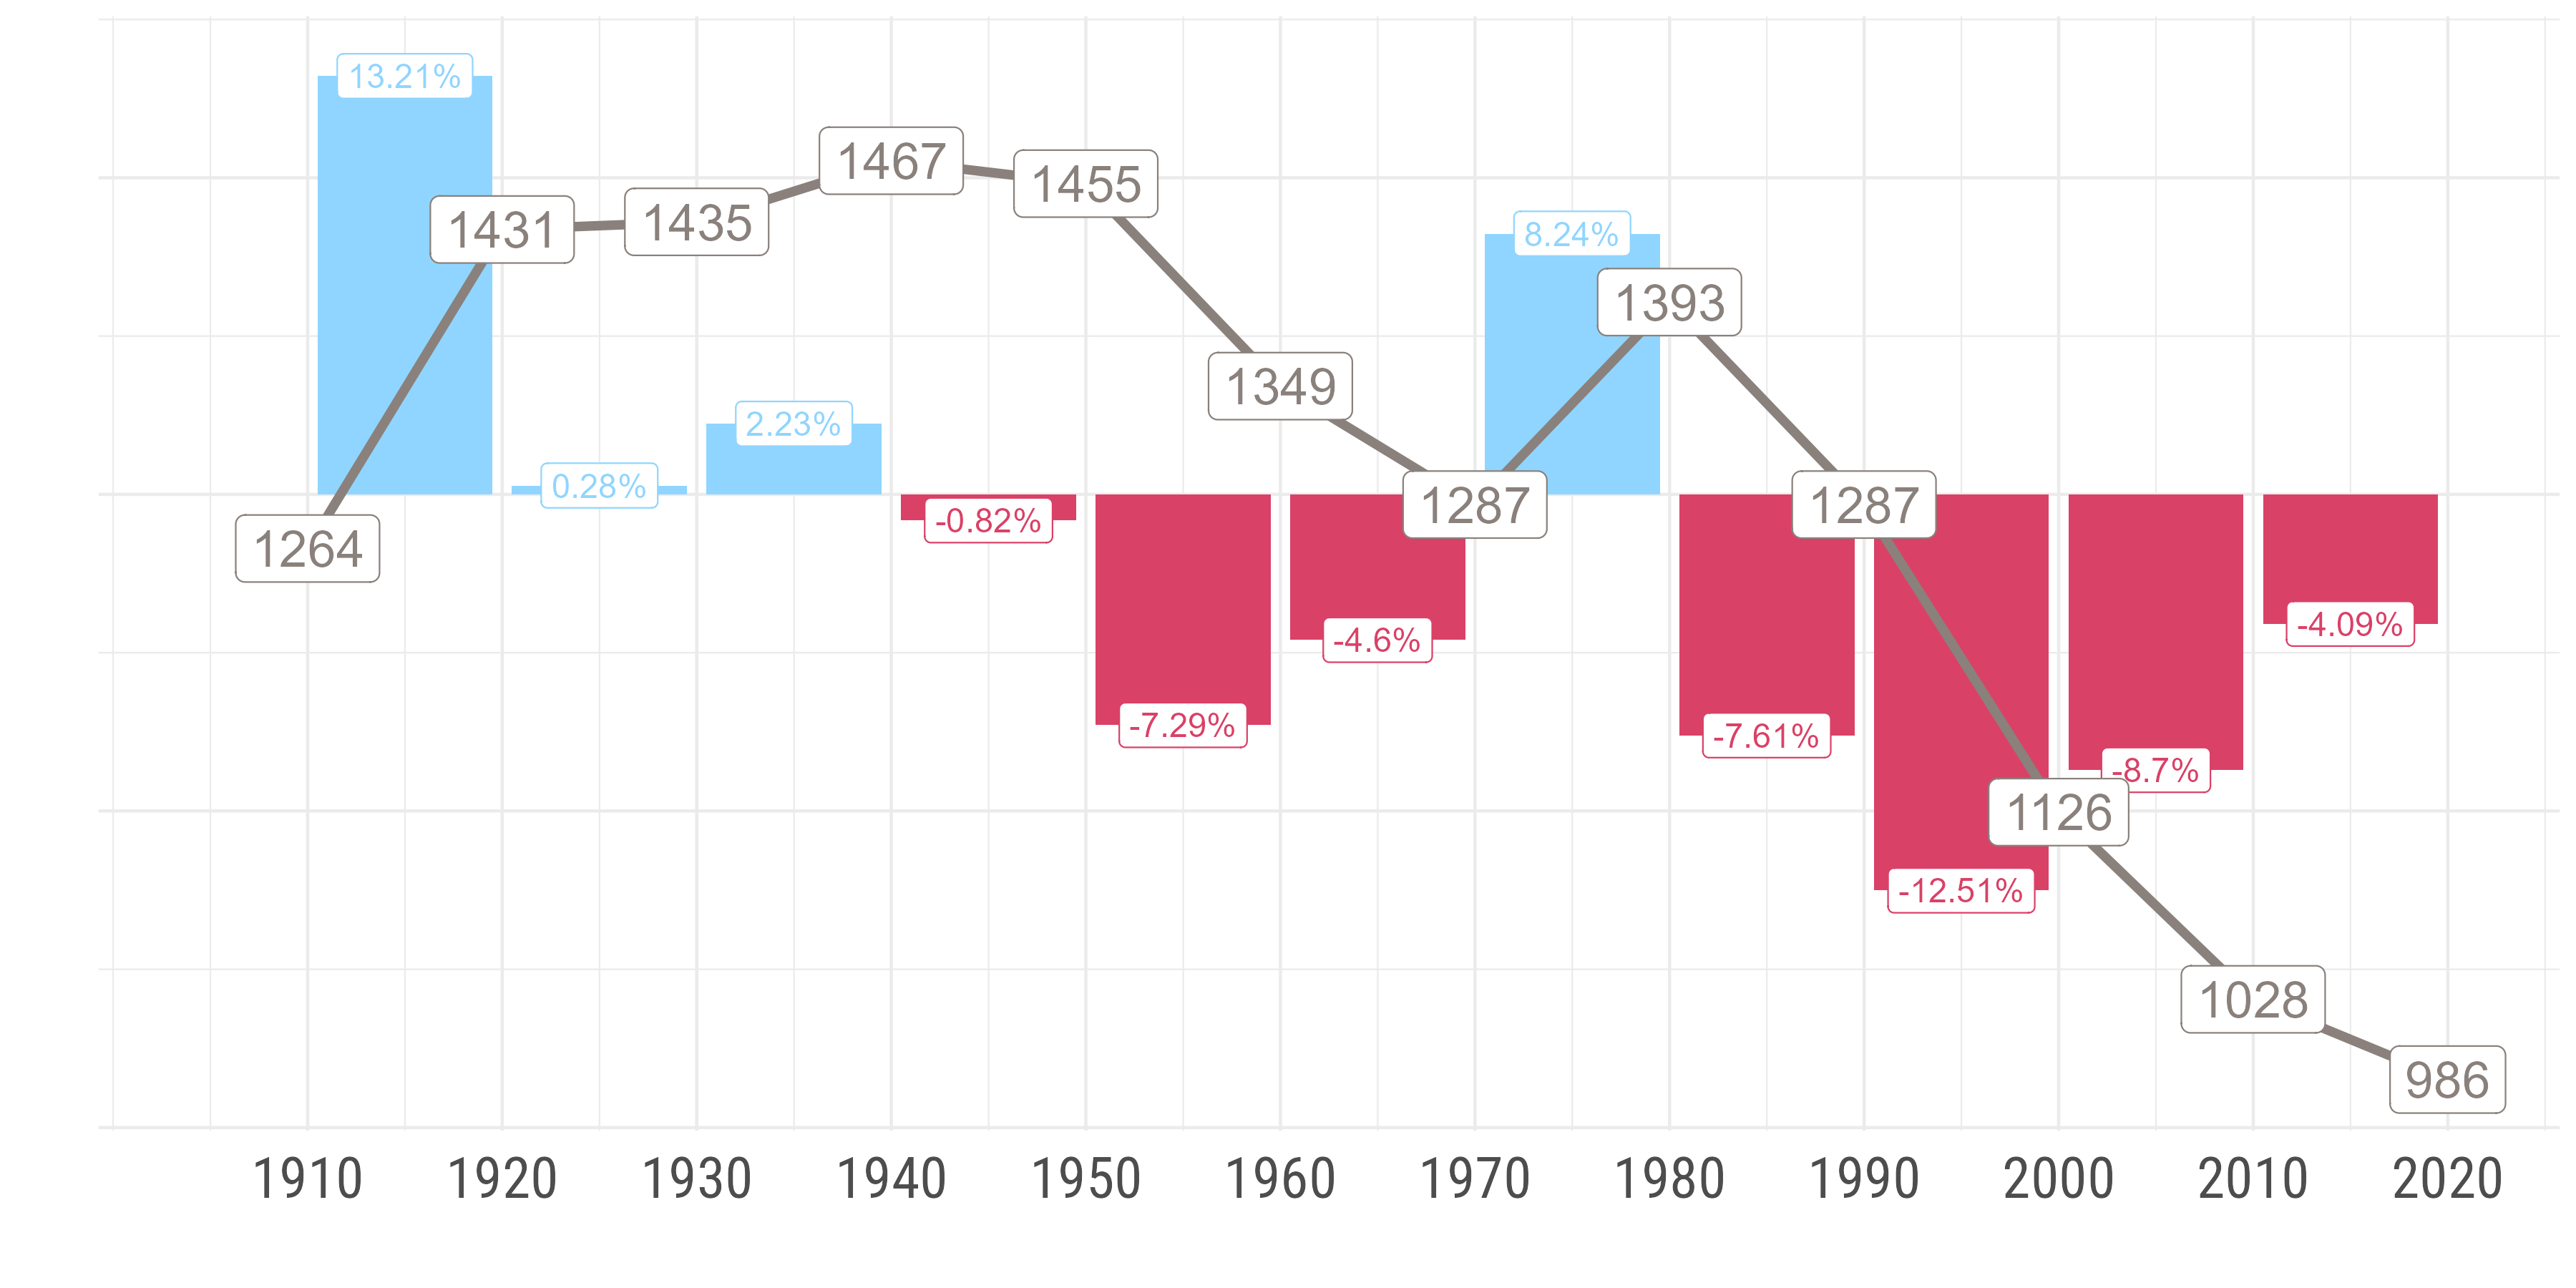
\includegraphics[width=\linewidth]{figures/historical_population_trends.png}
    \rule[-5pt]{\linewidth}{0.4pt}
    \floatnote{Data come from the \href{https://www.unomaha.edu/college-of-public-affairs-and-community-service/center-for-public-affairs-research/programs/nebraska-state-data-center.phpl}{University of Nebraska-Omaha Data Center} and the \href{https://www.census.gov/programs-surveys/decennial-census.html}{Decennial Census}.}
\end{framed}
\end{figure}

% \subsection{Population Projections}

\noindent \textbf{Figure~\ref{fig:populationProjections}} presents several possible population scenarios for Bloomfield. There are many unknown factors that can affect future growth projections. However, many organizations rely on using historical trends as the basis for forecasting future growth or decline.\\

\begin{figure}[H]
\centering
\begin{framed}
    \caption{Population Projections for Bloomfield, Nebraska}
    \label{fig:populationProjections}
    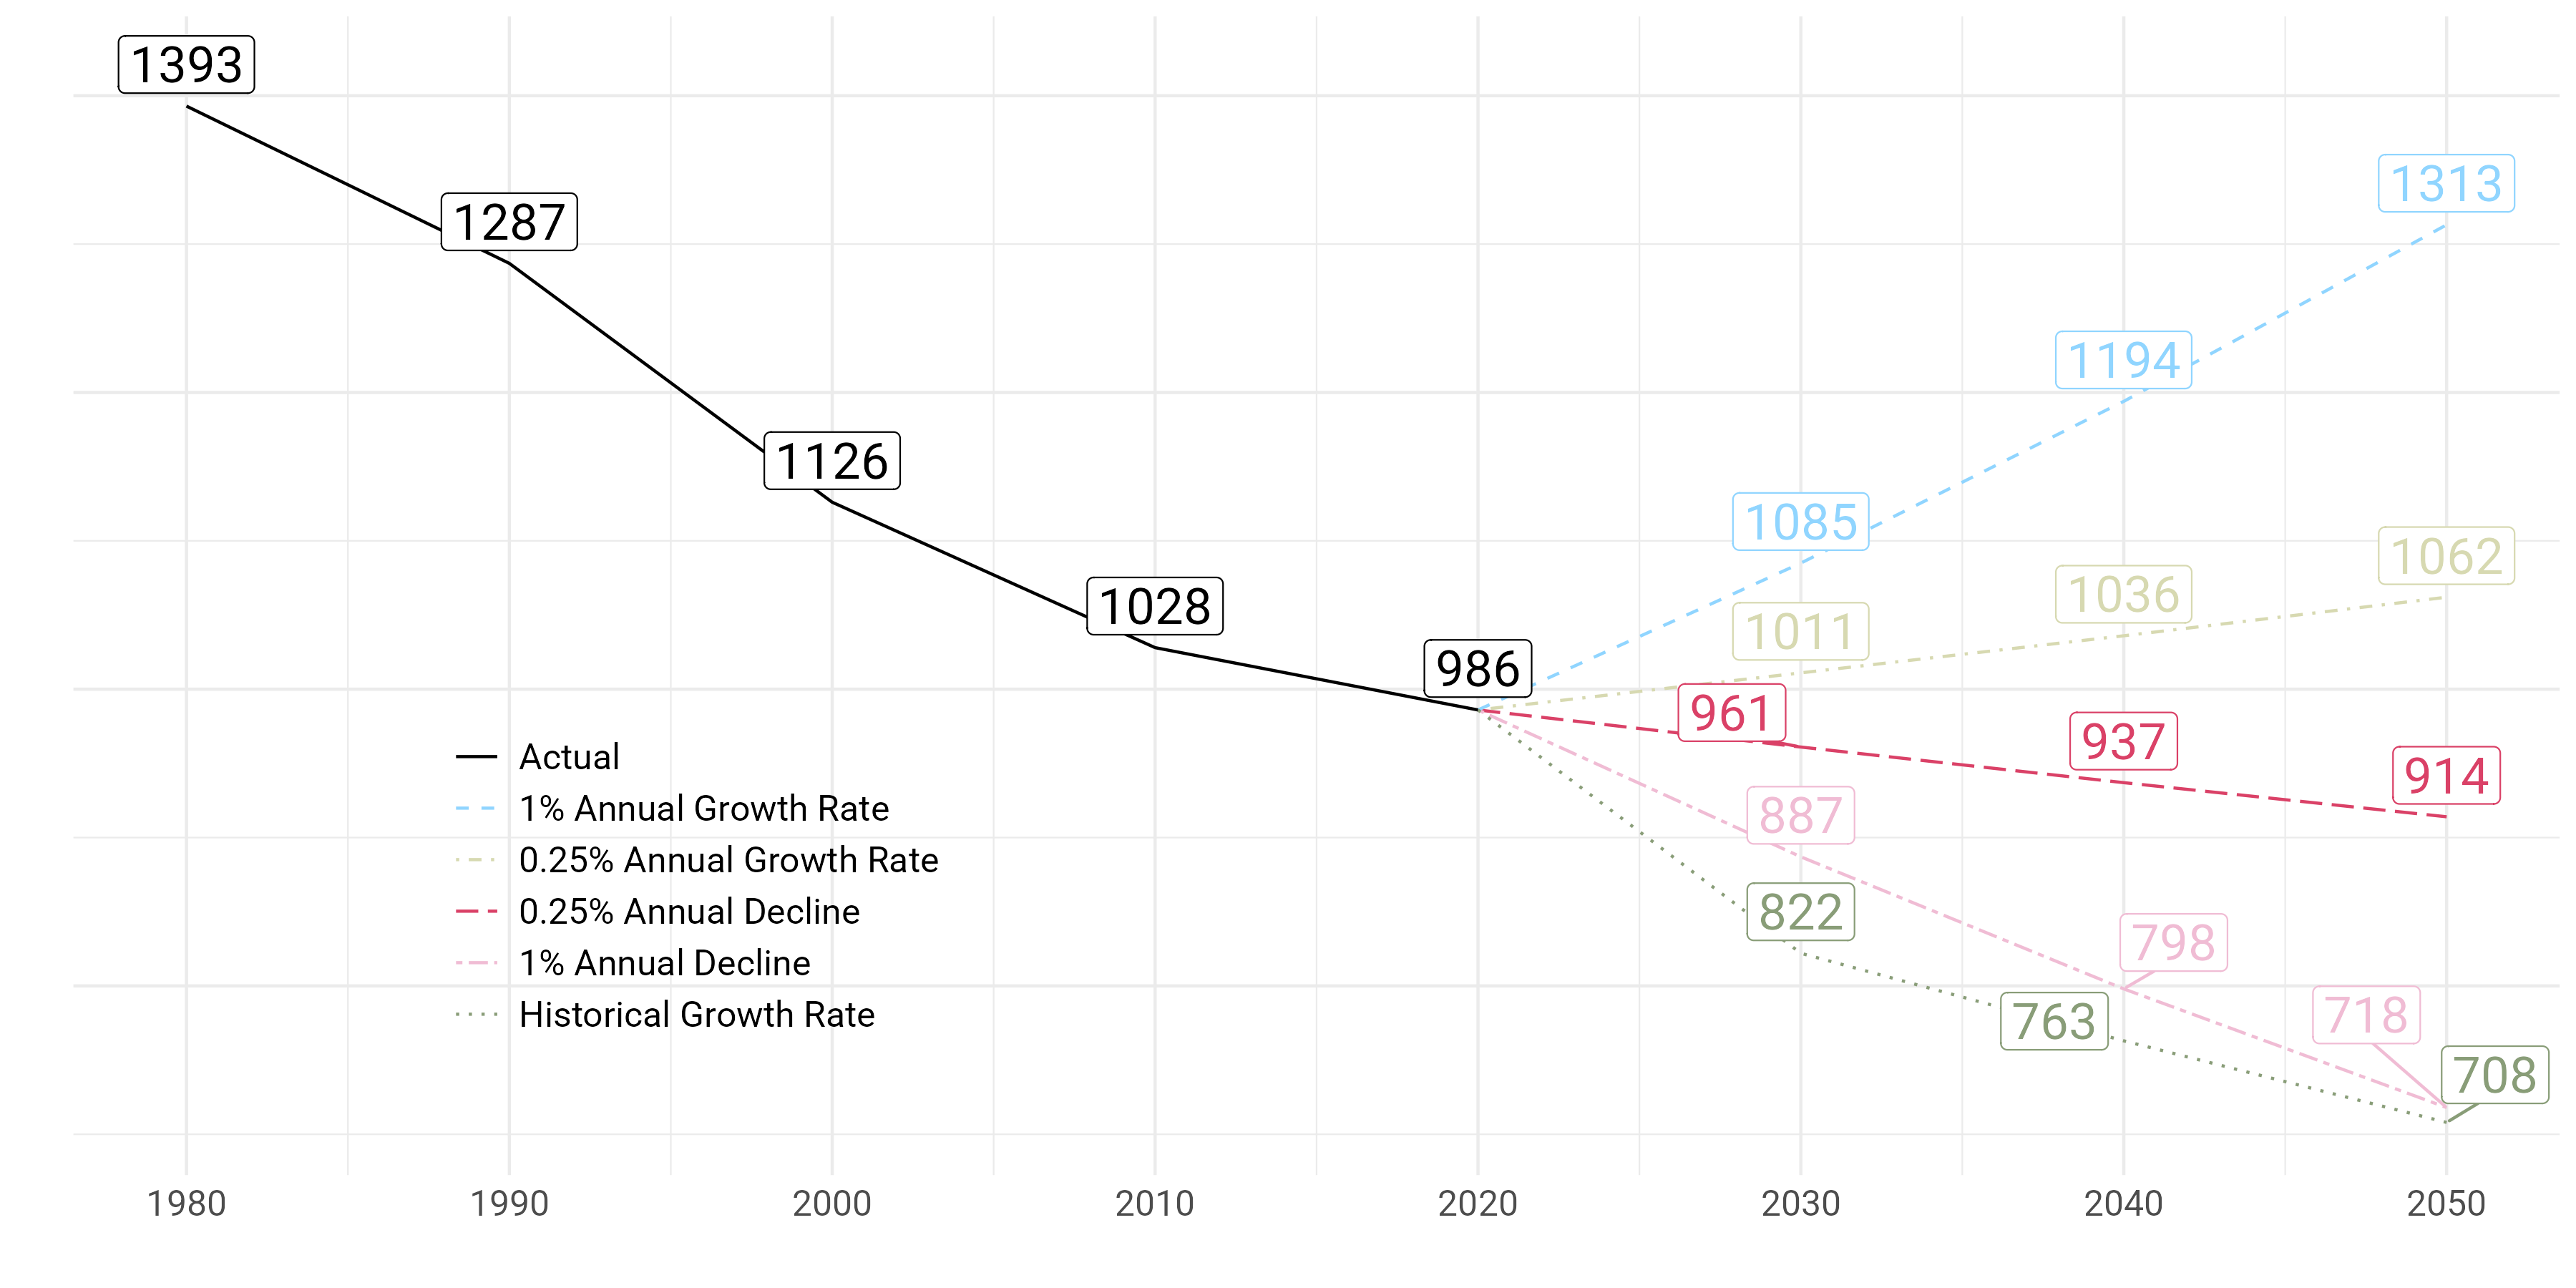
\includegraphics[width=\linewidth]{figures/population_projections.png}
    \rule[-5pt]{\linewidth}{0.4pt}
    \floatnote{Data come from the \href{https://www.unomaha.edu/college-of-public-affairs-and-community-service/center-for-public-affairs-research/programs/nebraska-state-data-center.phpl}{University of Nebraska-Omaha Data Center} and the \href{https://www.census.gov/programs-surveys/decennial-census.html}{Decennial Census}.}
\end{framed}
\end{figure}

\noindent Some projections indicate future growth for Bloomfield, while others -- including the historical one -- suggest continued decline. However, if Bloomfield's population grows, the city will need to add additional housing units. This will require the new development of adjacent lands and possible redevelopment of lands already in the city. \textbf{Table~\ref{table:populationProjections}} uses the 2023 ACS estimate of 2.04 persons per household to document projected needs.

\begin{table}[H] 
\begin{framed}
\centering \doublespacing
  \caption{Population Projection Scenarios and Housing Needs}
  \label{table:populationProjections}
 \scalebox{0.85}{
\begin{tabular}{l D{.}{.}{8.5} D{.}{.}{8.5}}
\hline \hline
& \multicolumn{1}{c}{\textbf{0.25\% Annual Growth Rate}} & \multicolumn{1}{c}{\textbf{1\% Annual Growth Rate}} \\ \hline
2040 Population Projection          & 1036  & 1194  \\
2050 Population Projection          & 1062  & 1313  \\
Total Population Increase by 2050   & 76    & 327   \\ \hline
New Housing Units Needed by 2050    & 38    & 161   \\
\hline
\end{tabular}
}
\floatnote{Data come from the \href{https://www.unomaha.edu/college-of-public-affairs-and-community-service/center-for-public-affairs-research/programs/nebraska-state-data-center.phpl}{University of Nebraska-Omaha Data Center}, the \href{https://www.census.gov/programs-surveys/decennial-census.html}{Decennial Census}, and the \href{https://www.census.gov/programs-surveys/acs.html}{2023 American Community Survey Five-Year Estimates}.}
\end{framed}
\end{table}

\pagebreak
\subsubsection*{Families and Households}
\noindent The Census defines a \textbf{family} as any two or more people (not necessarily including a householder) residing together and related by birth, marriage, or adoption. A \textbf{household} consists of one or more persons residing together who may or may not be related by birth, marriage, or adoption. Multiple families can reside in the same household.\\

\noindent \textbf{Figure~\ref{fig:householdSize}} is based on estimates from the 2023 U.S. Census American Community Survey and shows how average family and household sizes have changed in Bloomfield over the past decade. The average family size has fluctuated but is now about the same as it was a decade prior, while the average household size has generally increased.

\begin{figure}[H]
\centering
\begin{framed}
    \caption{Average Family and Household Sizes, 2013-2023}
    \label{fig:householdSize}
    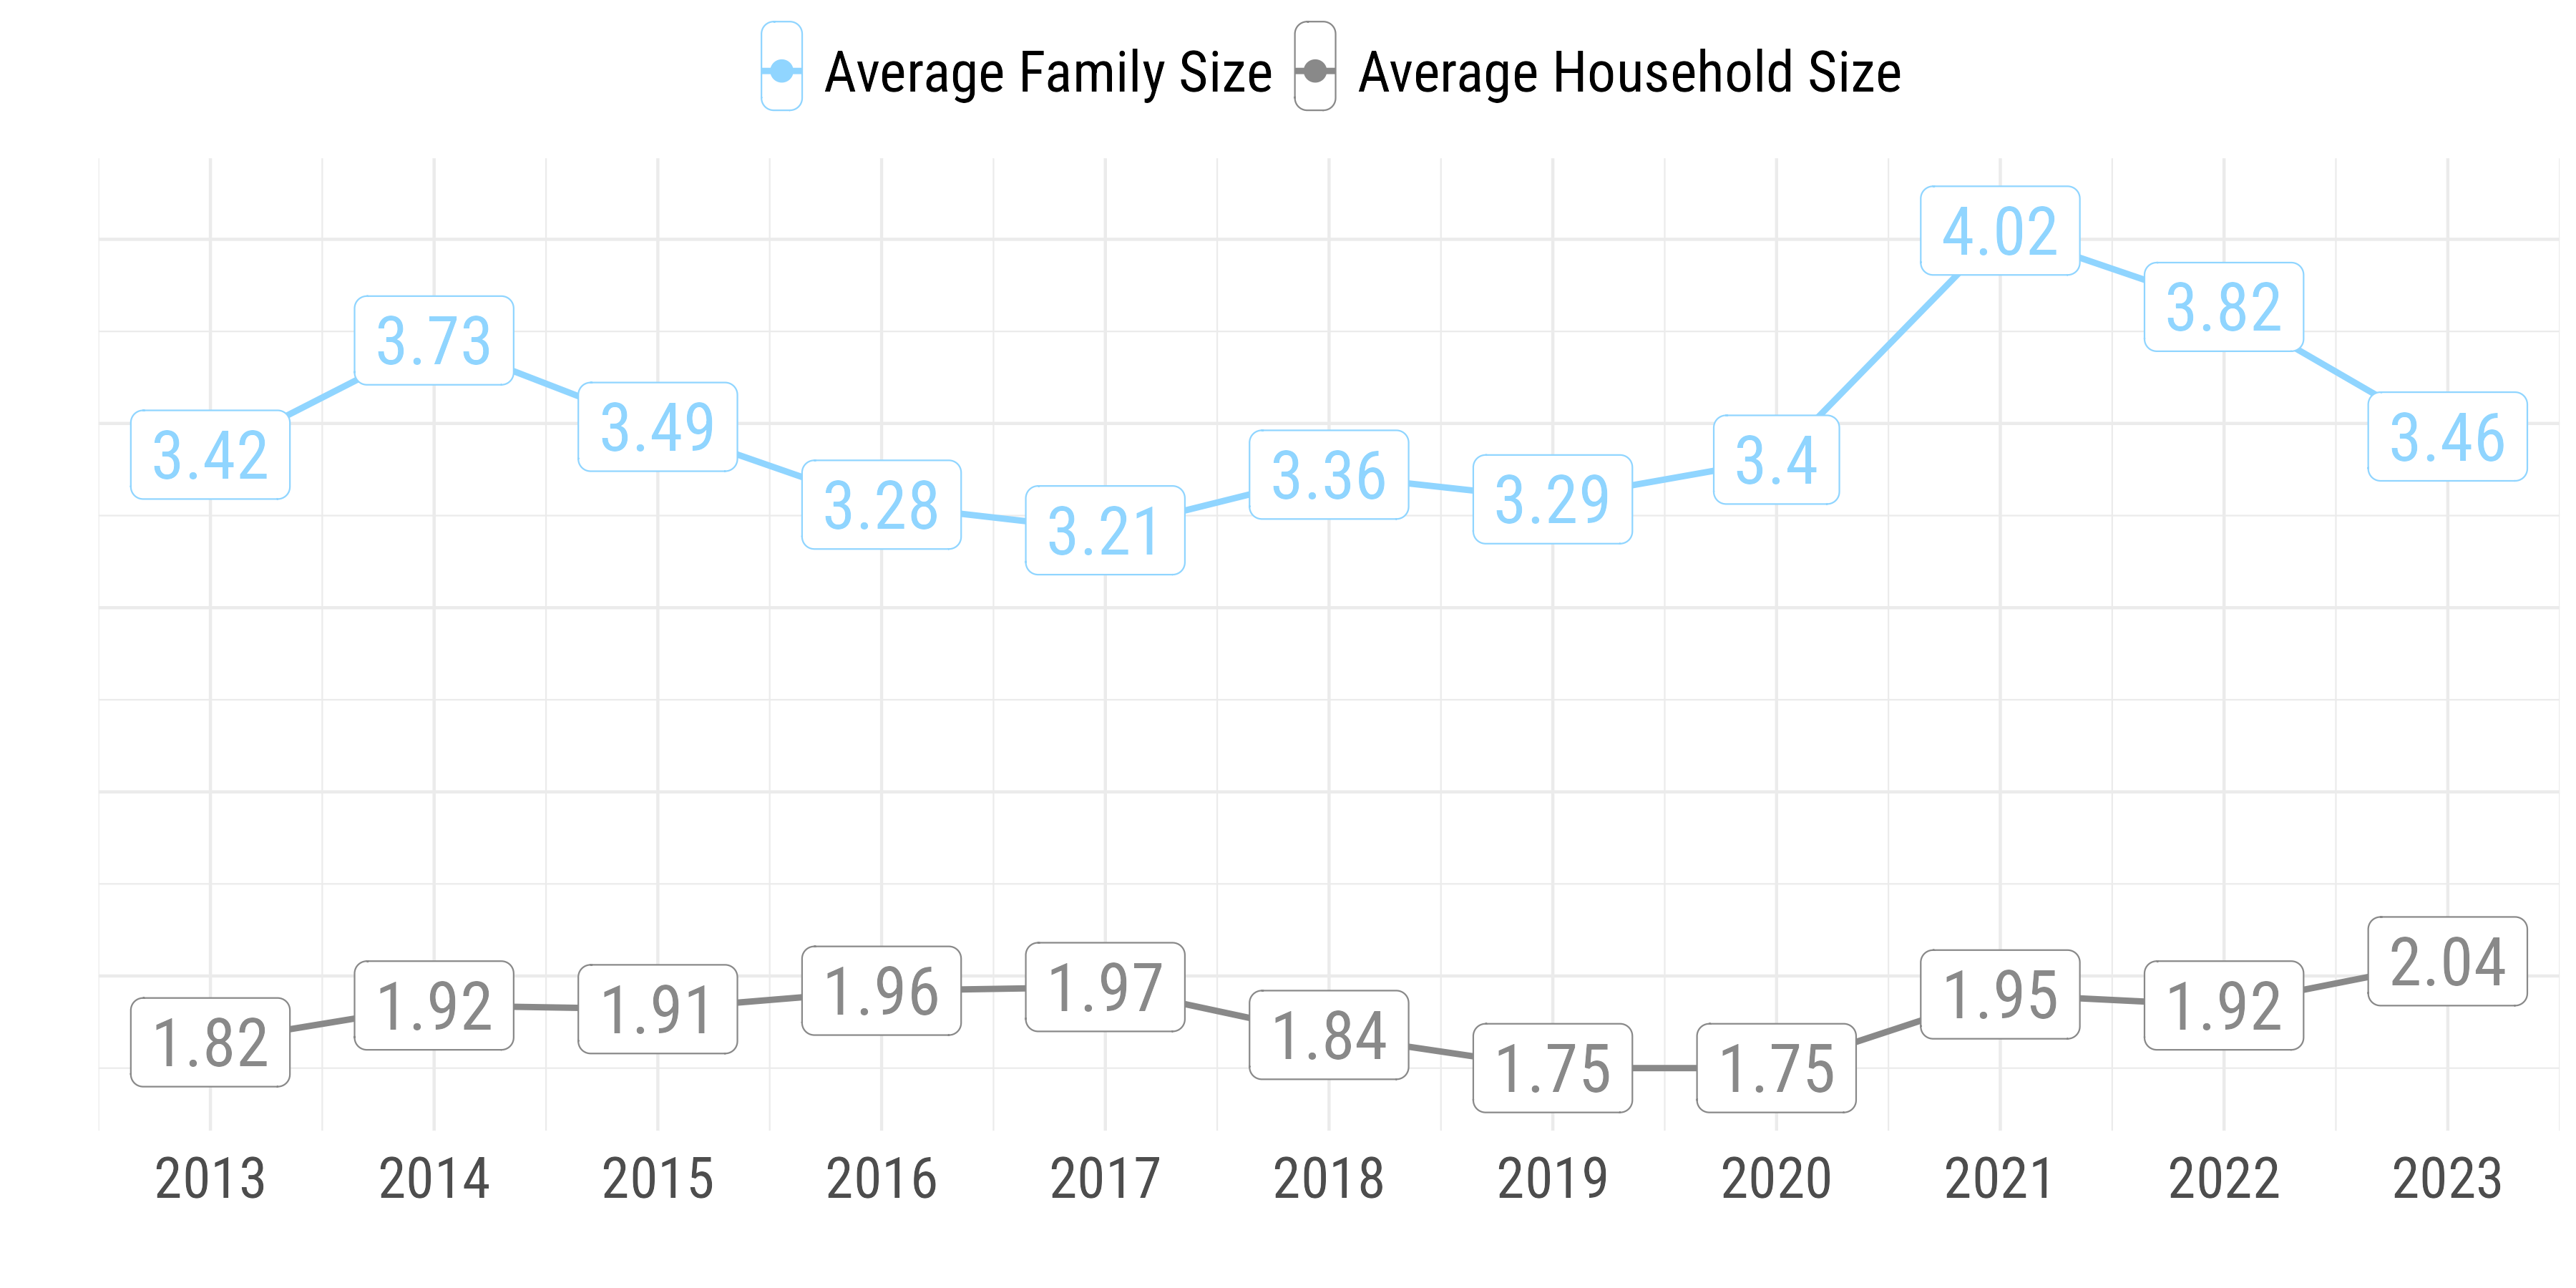
\includegraphics[width=\linewidth]{figures/household_size.png}
    \rule[-5pt]{\linewidth}{0.4pt}
    \floatnote{Data come from the \href{https://www.census.gov/programs-surveys/acs.html}{2013 through 2023 American Community Survey Five-Year Estimates}.}
\end{framed}
\end{figure}

\pagebreak
\subsubsection*{Median Age}

\noindent Bloomfield's population has steadily aged. \textbf{Figure~\ref{fig:medianAge}} shows how, between 2017 and 2019, the median age in Bloomfield jumped more than five years, and has steadily remained at just below sixty ever since.

\begin{figure}[H]
\centering
\begin{framed}
    \caption{Median Age, 2013-2023}
    \label{fig:medianAge}
    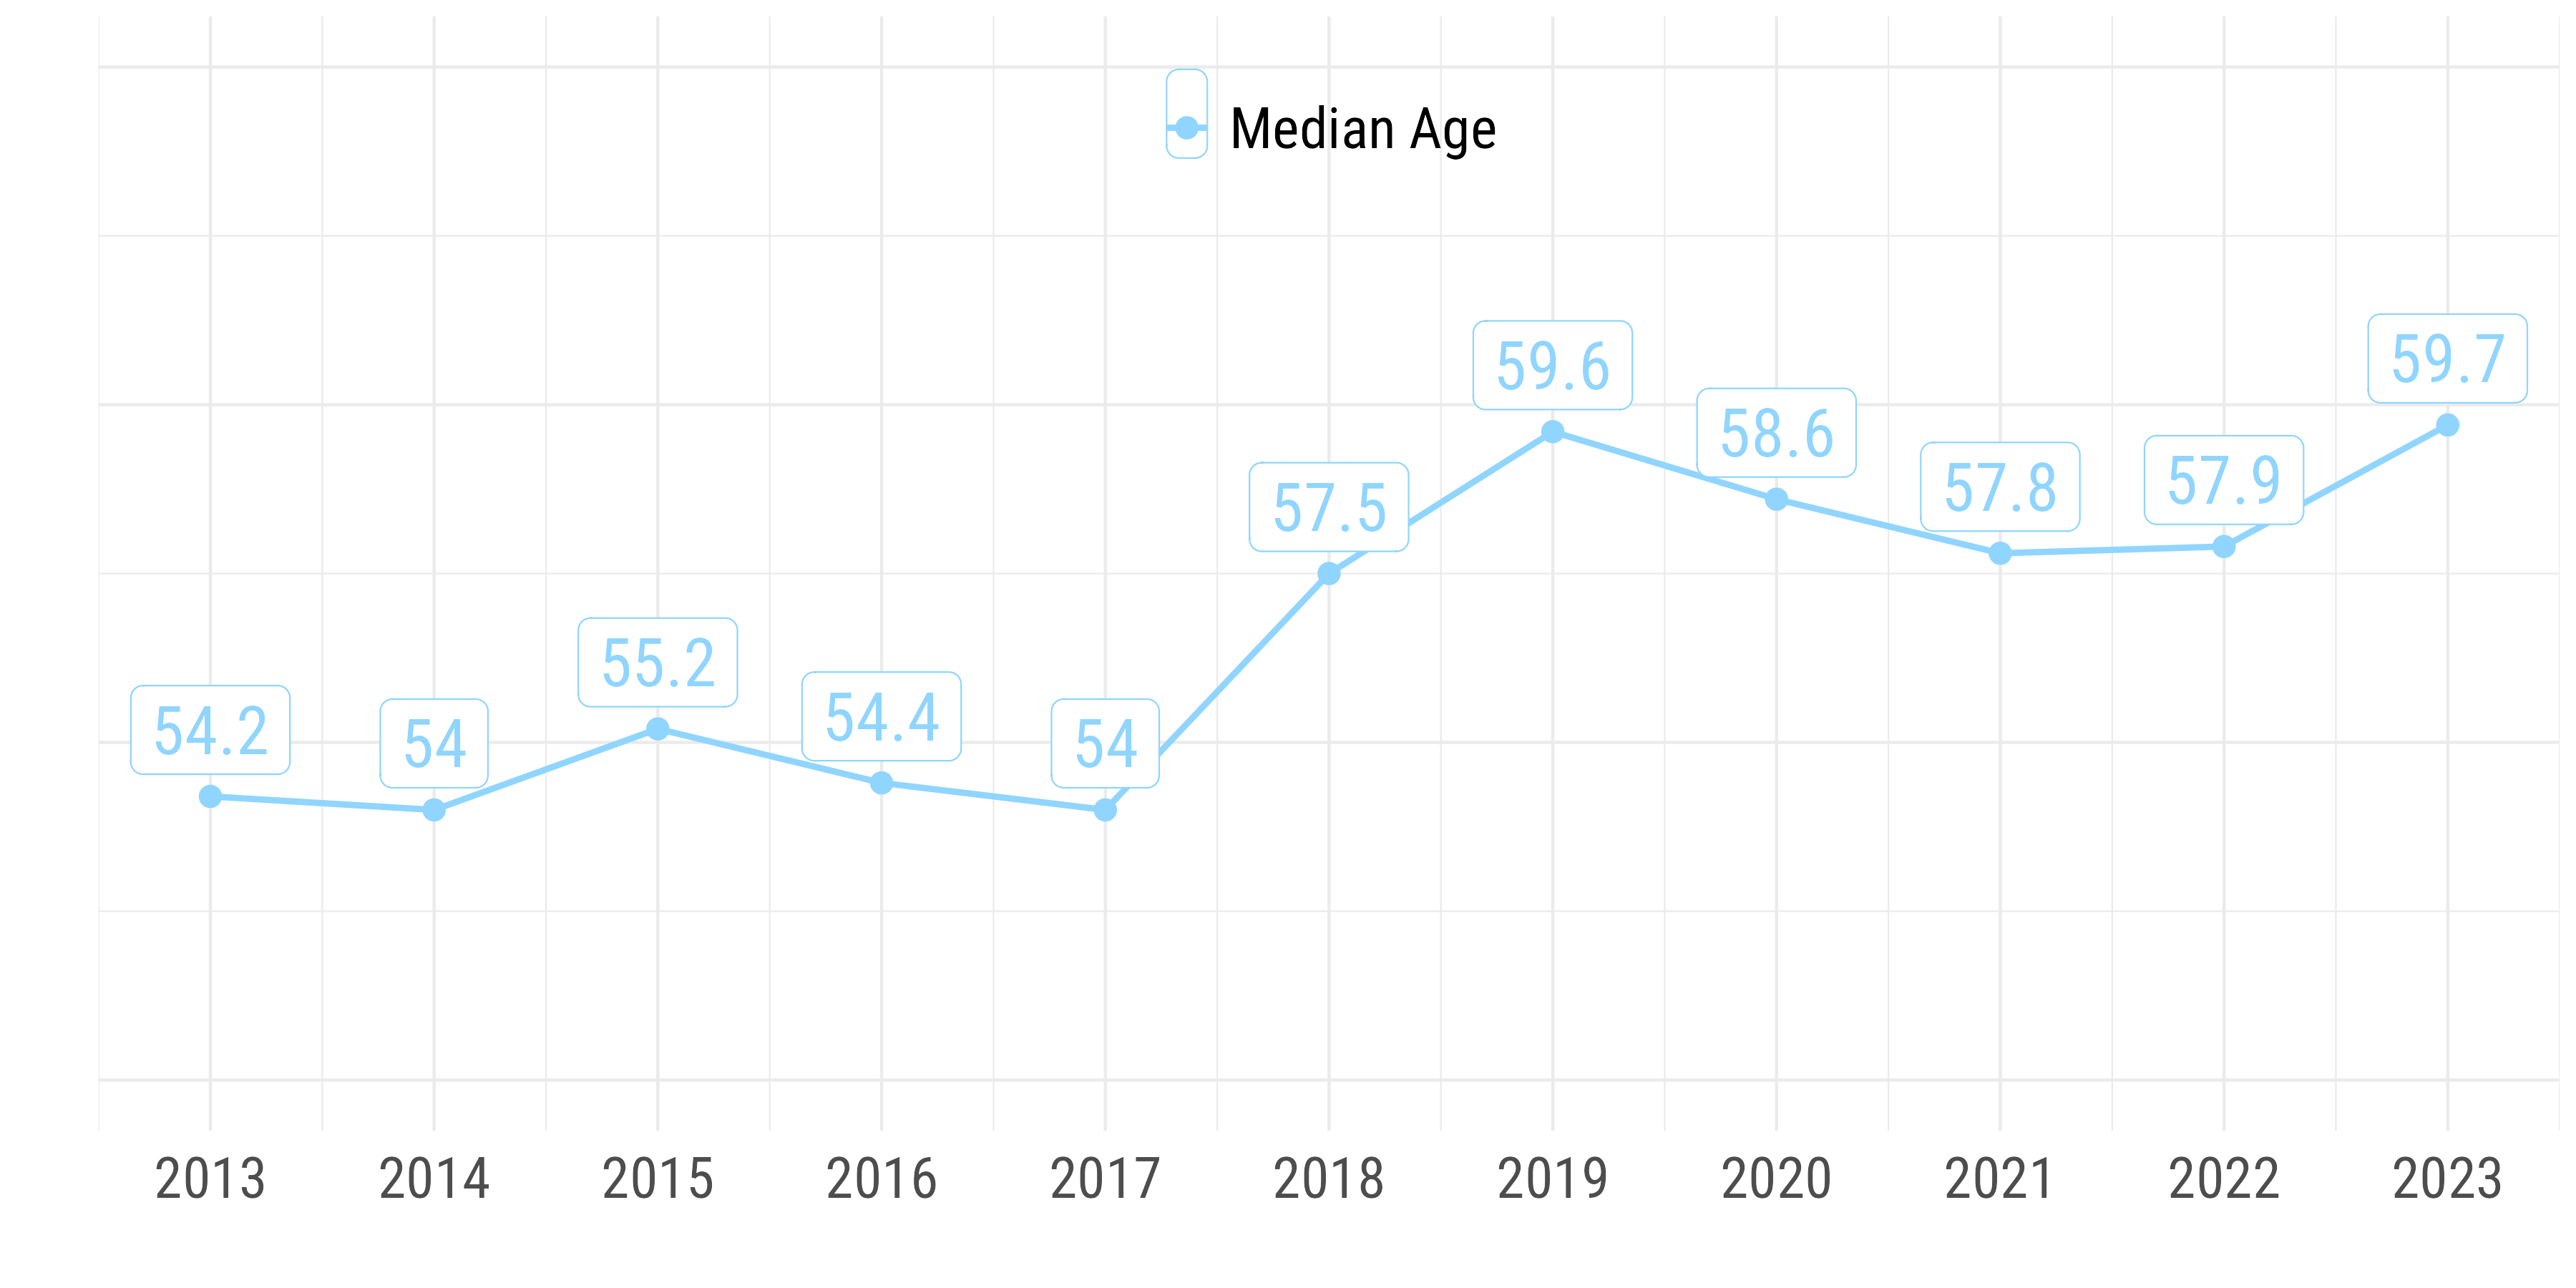
\includegraphics[width=\linewidth]{figures/median_age.png}
    \rule[-5pt]{\linewidth}{0.4pt}
    \floatnote{Data come from the \href{https://www.census.gov/programs-surveys/acs.html}{2013 through 2023 American Community Survey Five-Year Estimates}.}
\end{framed}
\end{figure}

\pagebreak
\subsubsection*{Housing Costs}

\noindent Overall, both incomes and costs of living have increased in Bloomfield over the last decade. \textbf{Figure~\ref{fig:housingCosts}} shows how, adjusting for inflation, each of median home values, median household incomes, and median gross rents in Bloomfield have slowly risen since 2013. However, much of that growth took place prior to 2020; over the last several years, these values have generally stagnated or even declined.

\begin{figure}[H]
\centering
\begin{framed}
    \caption{Housing Costs for Bloomfield, Nebraska}
    \label{fig:housingCosts}
    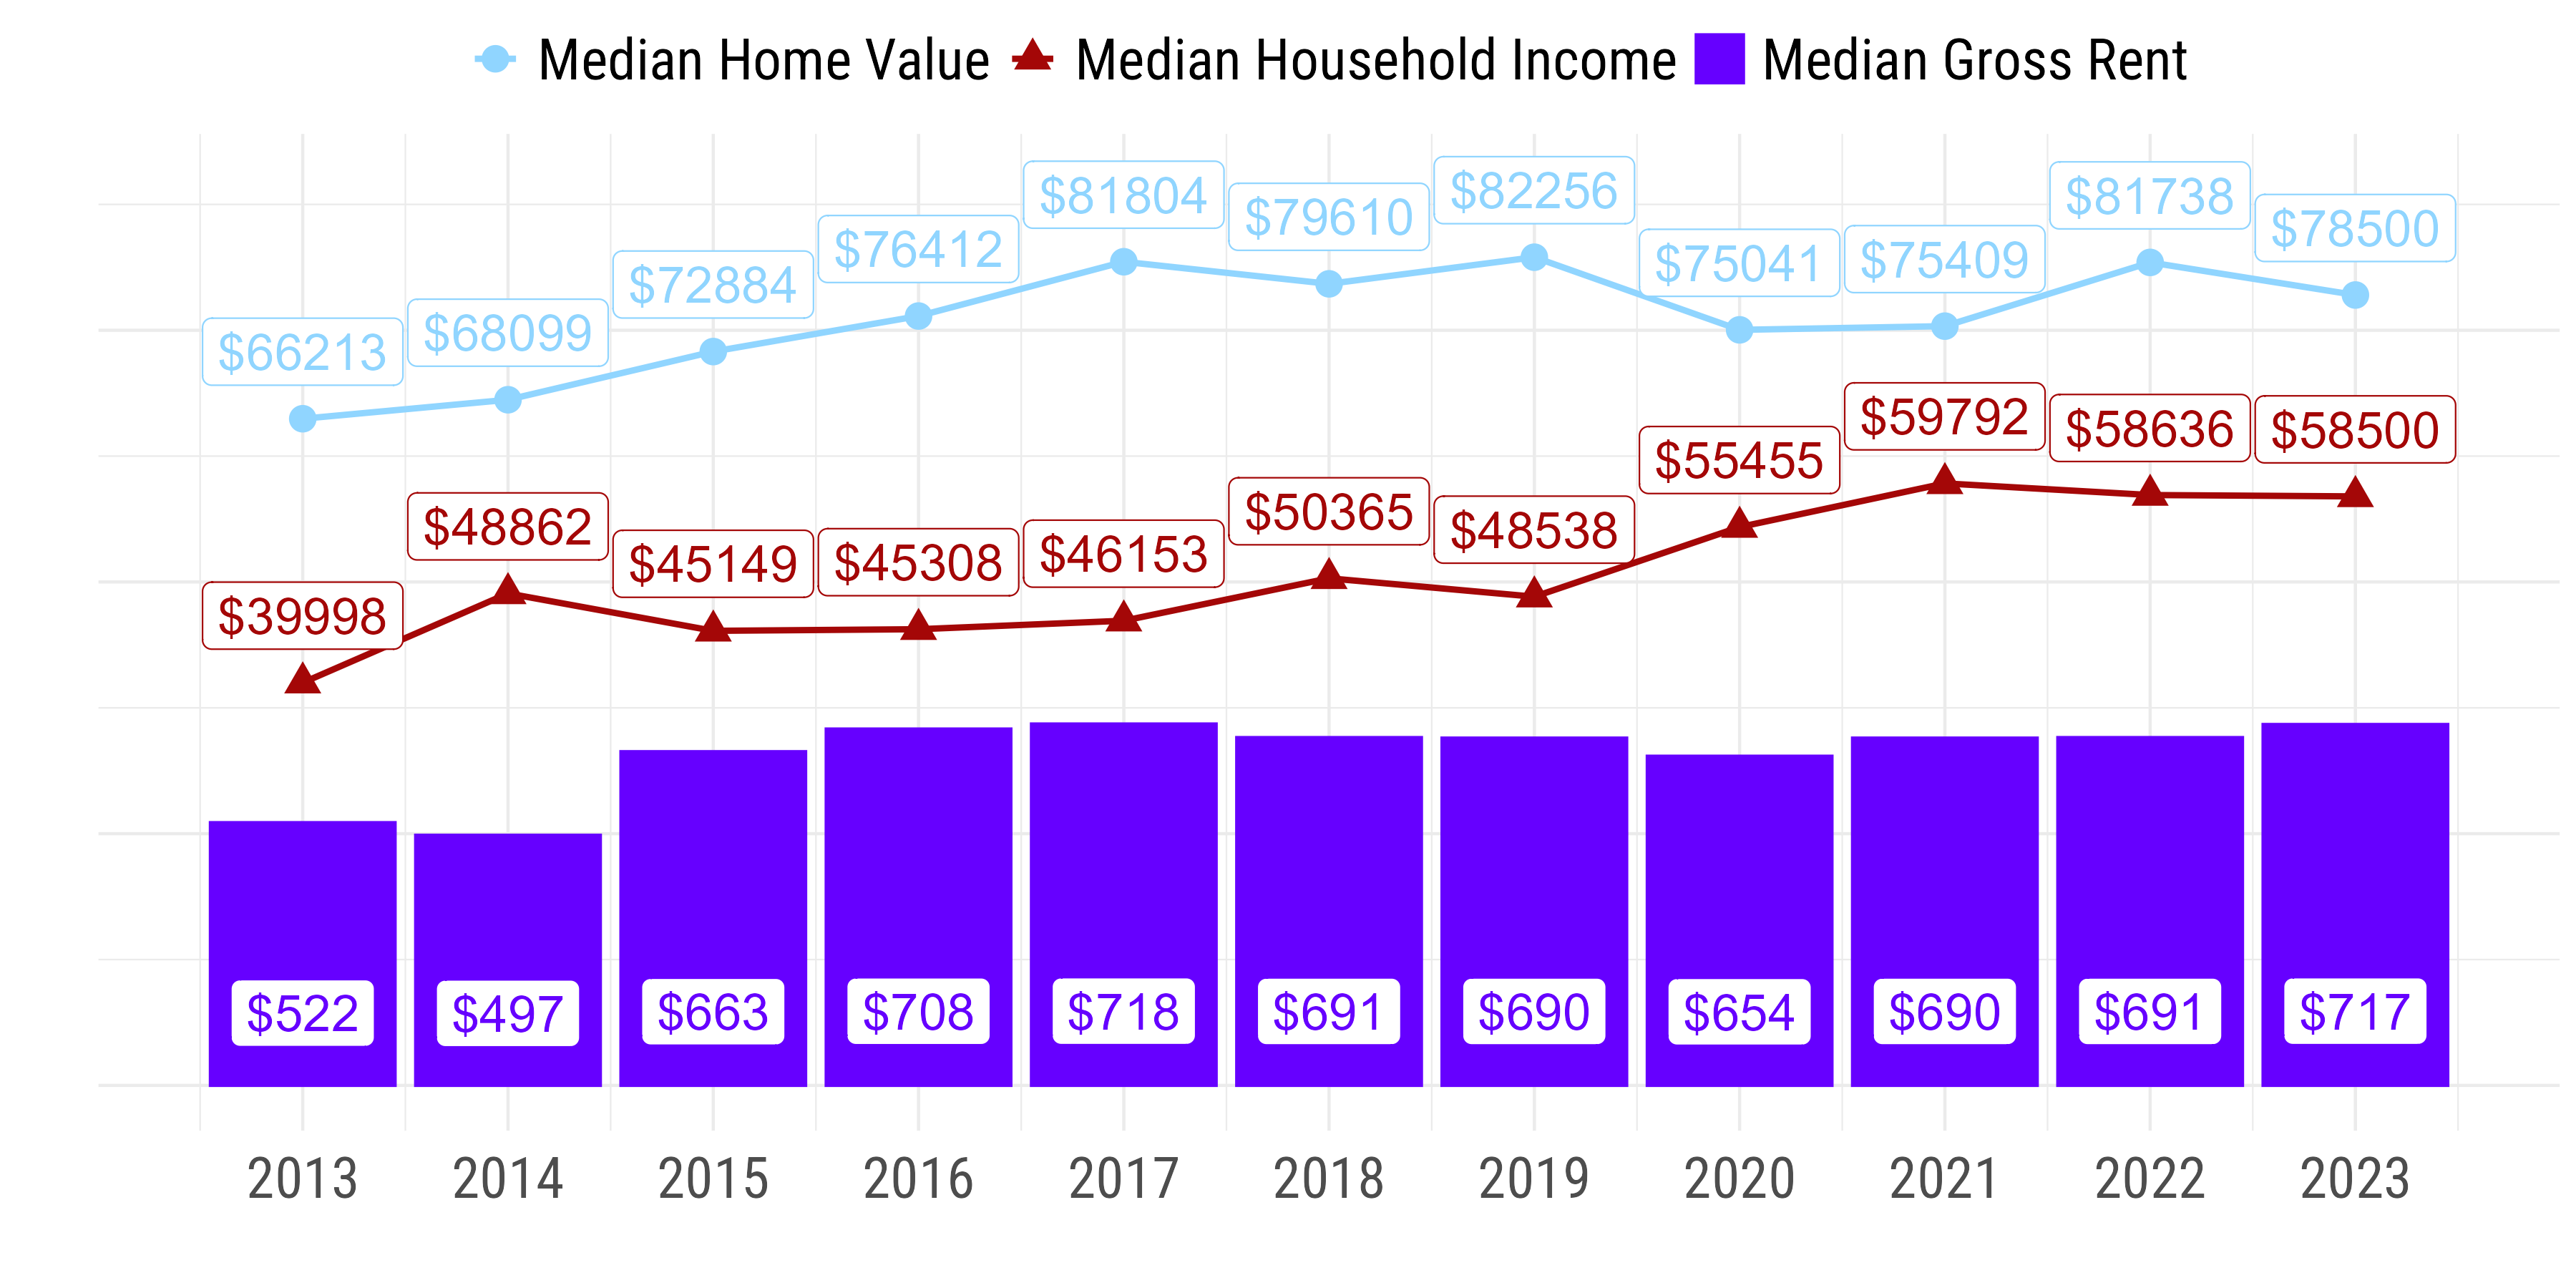
\includegraphics[width=\linewidth]{figures/housing_costs.png}
    \rule[-5pt]{\linewidth}{0.4pt}
    \floatnote{Data come from the \href{https://www.census.gov/programs-surveys/acs.html}{2013 through 2023 American Community Survey Five-Year Estimates}. Units are in 2023-adjusted real dollars.}
\end{framed}
\end{figure}

\pagebreak
\noindent Respondents to the community survey tend to be more affluent than the ACS would suggest. Fully two-thirds of respondents indicated that they have incomes above the Bloomfield median. Of that two-thirds, about half reported household incomes more than \$100,000. \textbf{Figure~\ref{fig:householdIncomes}} documents this distribution.

\begin{figure}[H]
\centering
\begin{framed}
    \caption{Household Incomes for Bloomfield, Nebraska}
    \label{fig:householdIncomes}
    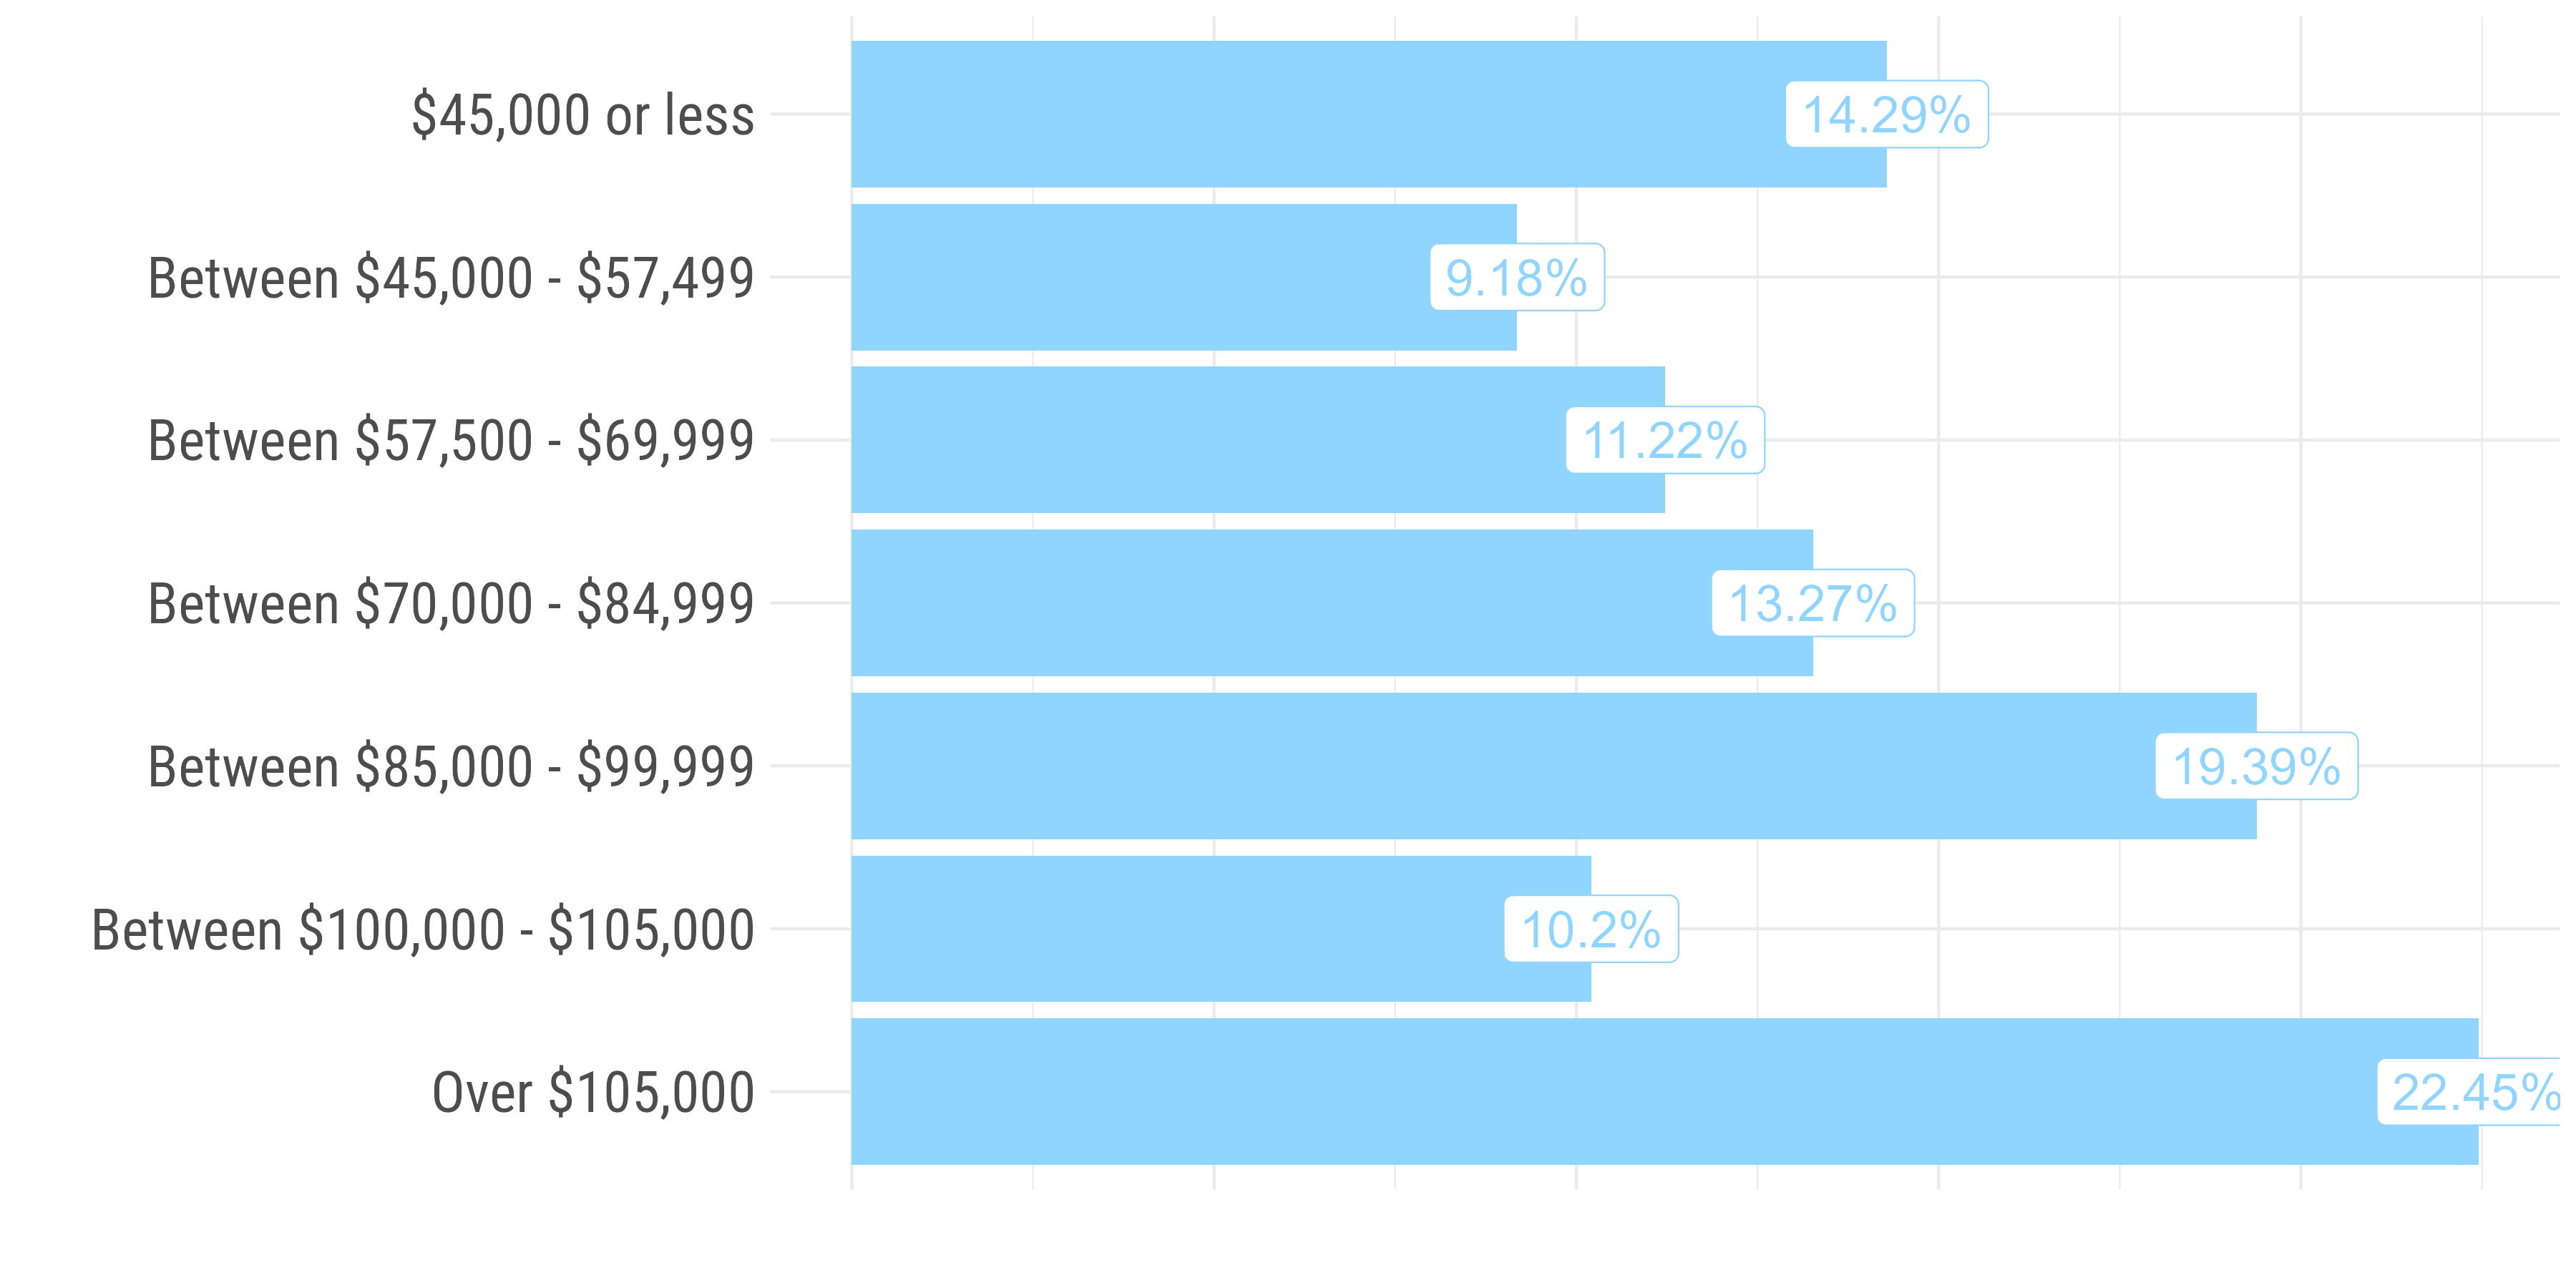
\includegraphics[width=\linewidth]{figures/survey_respondent_incomes.png}
    \rule[-5pt]{\linewidth}{0.4pt}
    % \floatnote{Data come from the \href{https://www.census.gov/programs-surveys/acs.html}{2013 through 2023 American Community Survey Five-Year Estimates}. Units are in 2023-adjusted real dollars.}
\end{framed}
\end{figure}

\pagebreak
\noindent Despite this, survey respondents experience housing situations close to the \href{https://www.hudexchange.info/programs/home/home-income-limits}{Department of Housing and Urban Development's (HUD) guidelines} that affordable housing costs no more than thirty percent of one's income. Per \textbf{Figure~\ref{fig:housingCostsSurvey}}, about seventy percent of Bloomfield respondents are at or above the thirty percent guideline.

\begin{figure}[H]
\centering
\begin{framed}
    \caption{Housing Costs for Bloomfield, Nebraska}
    \label{fig:housingCostsSurvey}
    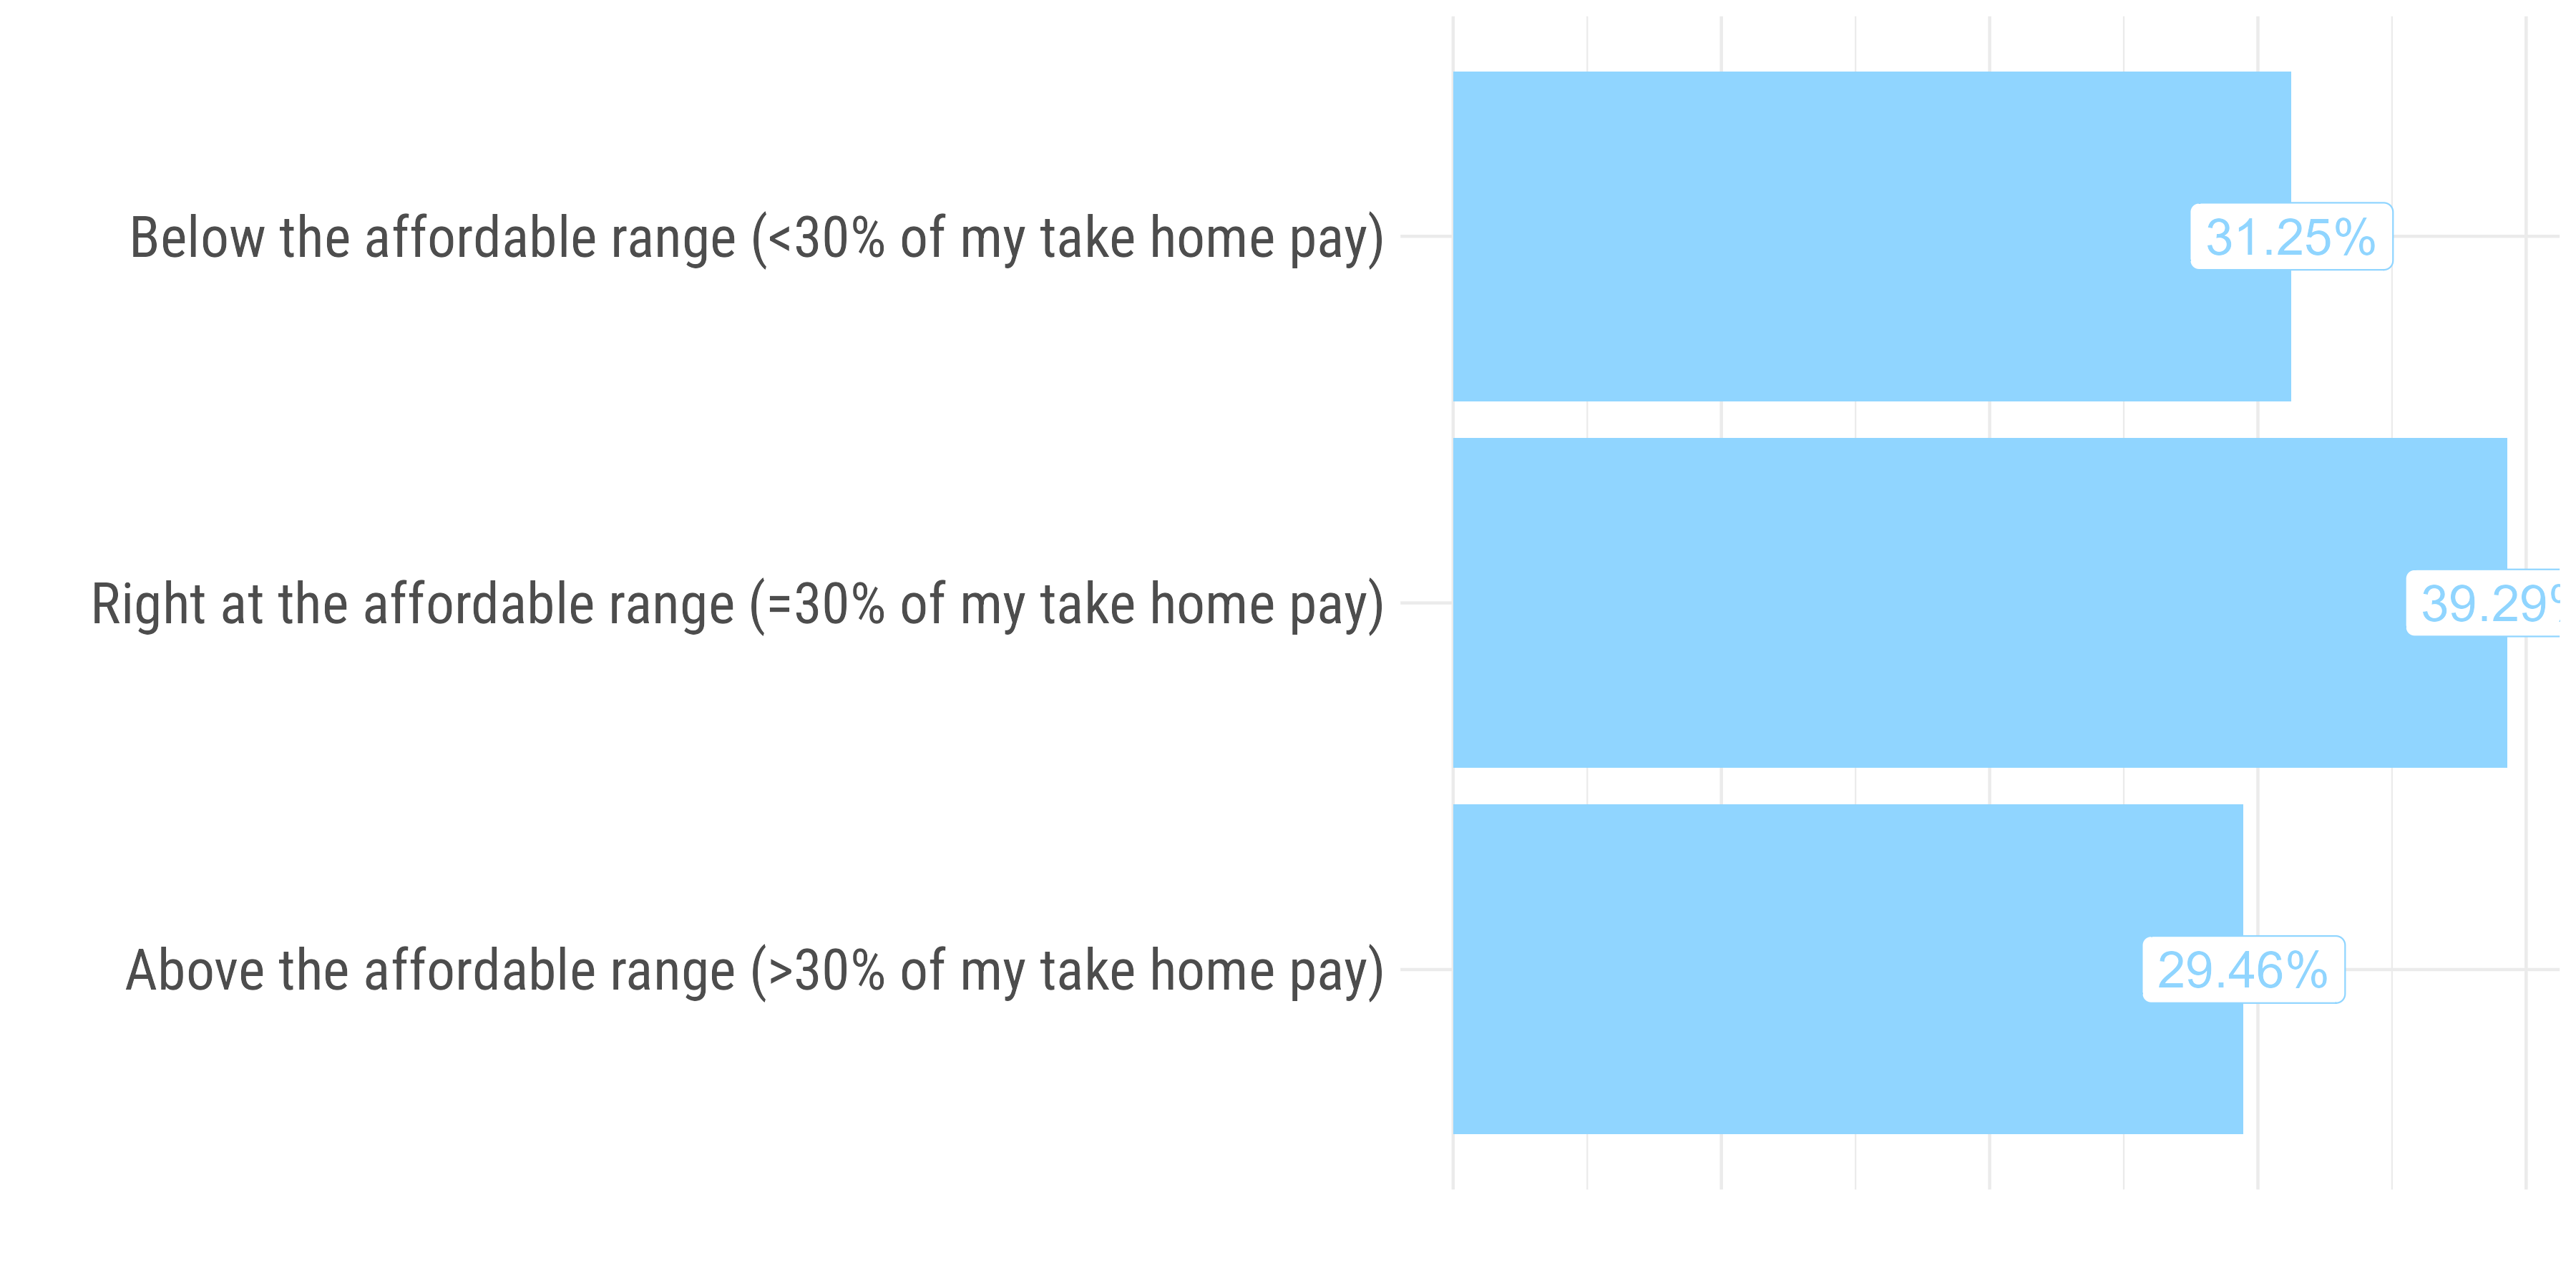
\includegraphics[width=\linewidth]{figures/survey_respondent_housing_costs.png}
    \rule[-5pt]{\linewidth}{0.4pt}
    % \floatnote{Data come from the \href{https://www.census.gov/programs-surveys/acs.html}{2013 through 2023 American Community Survey Five-Year Estimates}. Units are in 2023-adjusted real dollars.}
\end{framed}
\end{figure}

\pagebreak
\subsection*{Key Takeaways}